% !TEX root = ./busty_transcription.tex
\section{Introduction}

Gene expression presides over much of the most important dynamism of living
organisms.   The level of expression of batteries of different genes is altered
as a result of spatiotemporal cues that integrate chemical, mechanical and other
types of signals.  The original repressor-operator model conceived by Jacob and
Monod in the context of bacterial metabolism has now been transformed into the
much broader subject of gene regulatory networks in living organisms of all
kinds~\cite{Jacob1961, Britten1969, Ben-TabouDe-Leon2007}.  One of the remaining
outstanding challenges to have emerged in the genomic era is our continued
inability to predict the regulatory consequences of different regulatory
architectures. This challenge stems first and foremost from our ignorance about
what those architectures even are with more than 60\% of the genes even in an
ostensibly well understood organism such as  {\it E. coli} with no regulatory
insights at all~\cite{Rydenfelt2014-2,Belliveau2018,Ghatak2019,
Santos_Zavaleta2019}. But even once we have established the identity of key
transcription factors and their binding sites of a given promoter architecture,
there remains the predictive challenge of understanding its input-output
properties, an objective that can be met by a myriad of approaches using the
tools of statistical physics~\cite{Ackers1982, Shea1985,
Buchler2003,Vilar2003a,Vilar2003b, Bintu2005a,Bintu2005c, Gertz2009,Sherman2012,
Saiz2013, Ko1991,Peccoud1995,Record1996, Kepler2001,
Sanchez2008,Shahrezaei2008,Sanchez2011, Michel2010}.  One root to such
predictive understanding is to focus on the simplest regulatory architecture and
to push the theory-experiment dialogue as far and as hard as it can be
pushed~\cite{Phillips2019}.  If we demonstrate that we can pass that test by
successfully predicting both the means and variance in gene expression, then
that provides a more solid foundation upon which to launch into more complex
problems.

To that end, in this paper we examine a wide variety of distinct models for the
simple repression regulatory architecture. This genetic architecture consists of
a DNA promoter regulated by a transcriptional repressor that binds to a single
binding site \cite{Garcia2011a}. All of the proposed models models coarse-grain
away some of the important microscopic features of this architecture that have
been elucidated by generations of geneticists, molecular biologists and
biochemists.
\mrm{Our aim is to understand the underlying principles of such coarse-graining
in order to increase the predictive power of these models. In doing so we hope
future models of regulatory response will be able to serve the powerful
predictive role needed to take synthetic biology from a brilliant exercise in
enlightened empiricism to a rational design framework as any other branch of
engineering.}
% Our aim is to understand the underlying principles of such
% coarse-graining such that future models of regulatory response can serve the
% powerful predictive role needed to take synthetic biology from what is often a
% brilliant exercise in enlightened empiricism and recast it as the same kind of
% rational design process we are used to in other branches of engineering. 
More precisely, we want phenomenology in the sense of coarse-graining away
atomistic detail, but still retaining biophysical meaning. For example, we are
not satisfied with the strictly phenomenological approach offered by the
commonly used Hill functions. Studies like~\cite{Razo-Mejia2018} have
demonstrated that Hill functions are clearly insufficient since each new
situation requires a completely new set of parameters. Such work requires a
quantitative theory of how biophysical changes at the molecular level propagate
to input-output functions at the genetic circuit level. We want concepts, not
mere facts. In particular a key question is: at this level of coarse graining,
what microscopic details do we need to explicitly model, and how do we figure
that out? For example, do we need to worry about all or even any of the steps
that individual RNAPs go through each time they make a transcript? Turning the
question around, can we see any imprint of those processes in the available
data? If the answer is no, then those processes are irrelevant for our purposes.
Forward modeling and inverse (statistical inferential) modeling are necessary to 
tackles such questions.

Figure~\ref{fig1:means_cartoons}(A) shows the qualitative picture of simple
repression that is implicit in the repressor-operator model. An operator, the
binding site on the DNA for a repressor protein, may be found occupied by a
repressor, in which case transcription is blocked from occurring. Alternatively,
that binding site may be found unoccupied, in which case RNA polymerase (RNAP)
may bind and transcription can proceed. The key assumption we make in this
simplest incarnation of the repressor-operator model is that binding of
repressor and RNAP in the promoter region of interest is exclusive, meaning that
one or the other may bind, but never may both be simultaneously bound. It is
often imagined that when the repressor is bound to its operator, RNAP is
sterically blocked from binding to its promoter sequence. Current evidence
suggests this is sometimes, but not always the case, and it remains an
interesting open question precisely how a repressor bound far upstream is able
to repress transcription. \marginpar{\it Cite that fig, from ??Nathan or Bill or
Rob??, showing locations of repressor binding sites far upstream of promoter}
Suggestions include ``action-at-a-distance'' mediated by kinks in the DNA,
formed when the repressor is bound, that prevent RNAP binding. Nevertheless, our
modeling in this work is sufficiently coarse-grained that we simply assume
exclusive binding and leave explicit accounting of these details out of the
problem.

\afterpage{\clearpage}
\begin{figure}[p]
\centering
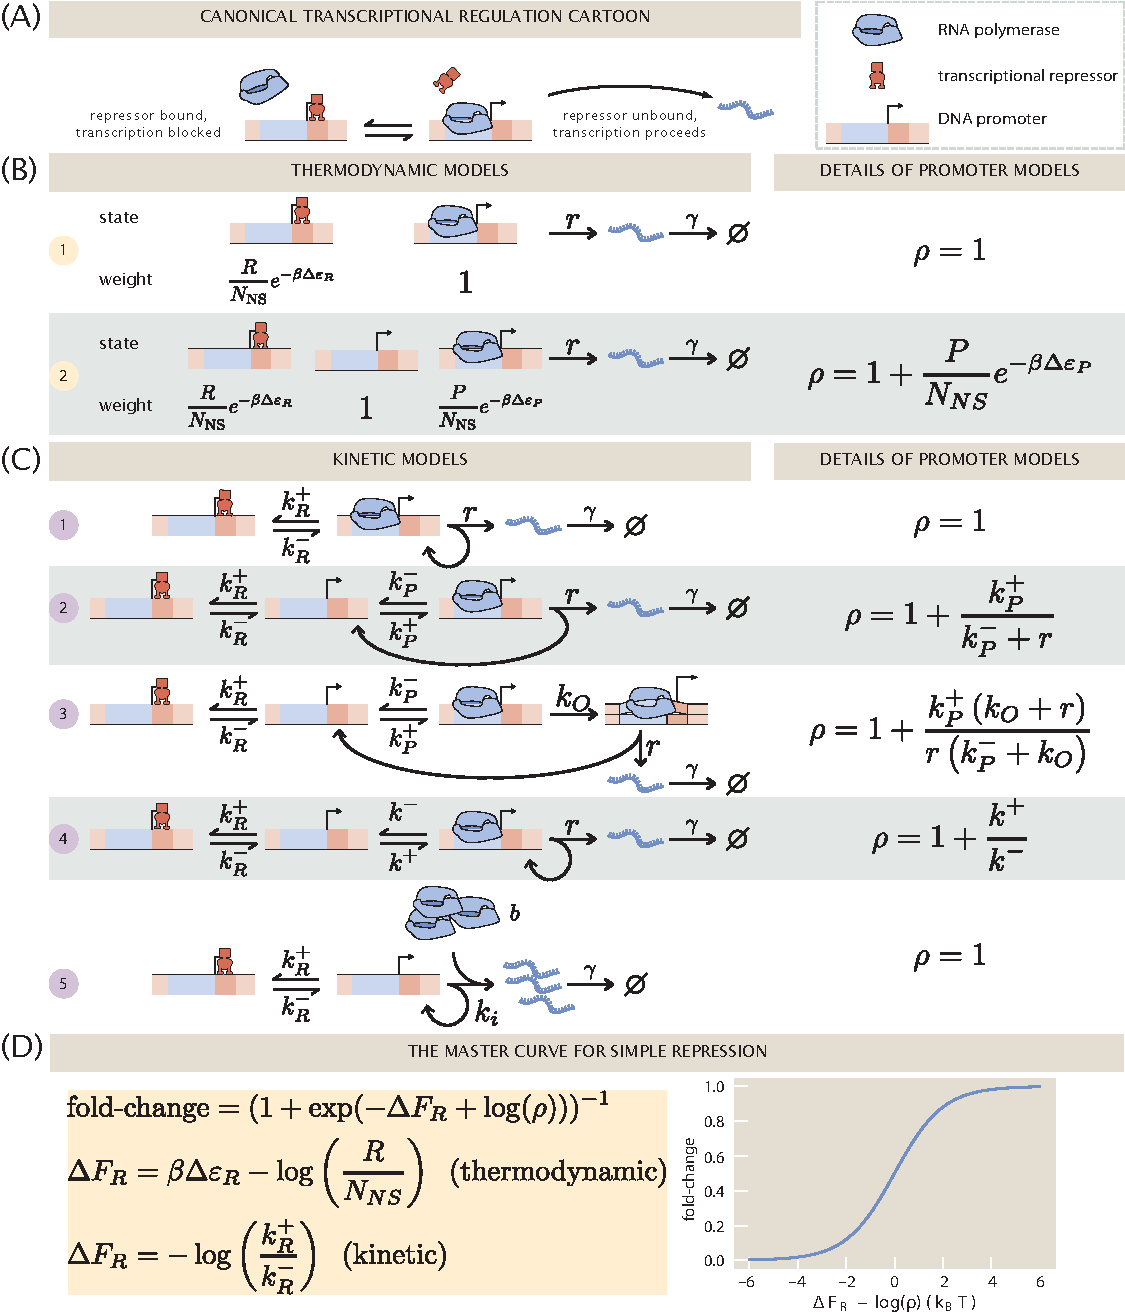
\includegraphics[width=\textwidth]{../figures/main/fig01.pdf}
\caption{\textbf{An overview of the simple repression motif at the level of
means.} (A) Schematic of the qualitative biological picture of the simple
repression genetic architecture. (B) and (C) A variety of possible
mathematicized cartoons of simple repression, along with the effective parameter
$\rho$ which subsumes all regulatory details of the architecture that do not
directly involve the repressor. (B) Simple repression models from an equilibrium
perspective. (C) Equivalent models cast in chemical kinetics language. (D) The
``master curve'' to which all cartoons in (B) and (C) collapse.}
\label{fig1:means_cartoons}
\end{figure}

The logic of the remainder of the paper is as follows. In
section~\ref{section_02_means}, we show how both thermodynamic models and
kinetic models based upon the chemical master equation all culminate in the same
underlying functional form for the fold-change in the average level of gene
expression as shown in Figure~\ref{fig1:means_cartoons}(D).
Section~\ref{section_03_beyond_means.tex} goes beyond an analysis of the mean
gene expression by asking how the same models presented in
Figure~\ref{fig1:means_cartoons}(C) can be used to explore noise in gene
expression. To make contact with experiment, all of these models must make a
commitment to some numerical values for the key parameters found in each such
model. Therefore in Section~\ref{section_04_bayesian_inference.tex} we explore
the use of Bayesian inference to establish these parameters and to rigorously
answer the question of how to discriminate between the different models.

%\mmnote{Key ideas, no particular order, that I haven't written down before:
%\begin{itemize}
%\item Our goal is to build phenomenological models of input-output functions of
%genetic circuits. More precisely, we want phenomenology in the sense of
%coarse-graining away atomistic detail, but still retaining biophysical meaning,
%e.g., we don't want to coarse-grain as far as Hill functions. Why not? We are
%motivated by studies like~\cite{Razo-Mejia2020}, for which Hill functions are
%insufficient. Such work requires a quantitative theory of how biophysical
%changes at the molecular level propagate to input-output functions at the
%genetic circuit level. We want concepts, not mere facts. In particular a key
%question is: at this level of coarse graining, what microscopic details do I
%need to explicitly model, and how do we figure that out? For example, do I need
%to worry about all or even any of the steps that individual RNAPs go through
%each time they make a transcript? Turning the question around, can we see any
%imprint of those processes in the available data? If the answer is no, then
%those processes are irrelevant for our purposes. Forward modeling and inverse
%(statistical inferential) modeling can complement each other beautifully here.
%\end{itemize}}

%Biochemistry tells us of a progression of steps, but theory tells us
%that coarse graining can be exact